\documentclass[12pt,a4paper]{article}
\usepackage[top=25.4mm, bottom=25.4mm, left=19.1mm, right=19.1mm]{geometry}


\usepackage[latin2]{inputenc}
\usepackage{graphicx}
\graphicspath{ {./images/} }
\usepackage{ulem}
\usepackage{amsmath}
\usepackage[document]{ragged2e}

\setlength{\parindent}{4em}
\setlength{\parskip}{1em}
\usepackage{hyperref}

\usepackage{fancyhdr}
\pagestyle{fancy}
\fancyhf{}
\fancyhead[LO]{\textbf{\small IoT and Smart Analytics}\\
\text{\small A Program by IIITH and TalentSprint}}

\usepackage{xcolor}
\usepackage{lipsum}

\rhead{\begin{picture}(0,0) \put(-250,-2){
\includegraphics[width=9cm]{EXP_08_Images/ts-iisc-logo-pr.png}} \end{picture}}
\cfoot{\thepage}


\begin{document}

\begin{center}

\textbf{\large \\EXPERIMENT 14 }\\[6pt]
\text{Using Arduino board as an AVR-ISP Programmer}
\end{center}

\textbf{\large LEARNING OBJECTIVES:}\\[3pt]
At the end of this experiment, participants will be able to:\vspace{-6mm}\begin{enumerate}
 \setlength\itemsep{-0.3em}
\item Understand \& use Arduino board as an AVR–ISP Programmer   \\
\end{enumerate}

\textbf{\large APPARATUS REQUIRED:}\\
\vspace{-3mm}
\begin{enumerate}
 \setlength\itemsep{-0.3em}
\item Arduino Uno board-2 pcs \\
\item USB cable-1pcs\\
\item Arduino IDE
\item LED-1pcs\\
\item Resistor 1k$\Omega$ -1pcs\\
\item Jumper wires\\

\end{enumerate}

\begin{justify}

\noindent \textbf{\large PROCEDURE}\\[3pt]
\textbf{Hardware and software setup : }\\
\textbf{A)	Making an Arduino as Programmer}\\[5pt]
Follow the steps below:\vspace{-6mm}
\begin{itemize}
\item Connect the Arduino board to the PC via USB that has to be used as a Programmer.
\item Go to the Arduino IDE $\rightarrow$ File Examples $\rightarrow$ & Arduino ISP $\rightarrow$ Arduino ISP.\\
Open this file and upload it in the Arduino (Programmer).
\item	Disconnect it from the PC. Label it as Programmer to recognize later.
\end{itemize}

\noindent \textbf{B) Programming the Target Arduino using Programmer}\\[5pt]
Follow the steps below:\vspace{-6mm}
\begin{itemize}
\item Take another Arduino as Target to be programmed and label it so that it can be recognized later.
\item Connect 5V and GND pins of both the Arduino one to one. Power is supplied through the programmer to the Target.
\item Connect pin 13(SCK), pin12 (MISO), and pin11 (MOSI) of both the Arduino one to one.
These connections are for communicating and data transfer from Programmer to Target.
\item Connect the Reset pin of the Target to pin10 of the Programmer. This is for avoiding continuously resetting. 


All the connections are shown in the figure given below:


\begin{center} 
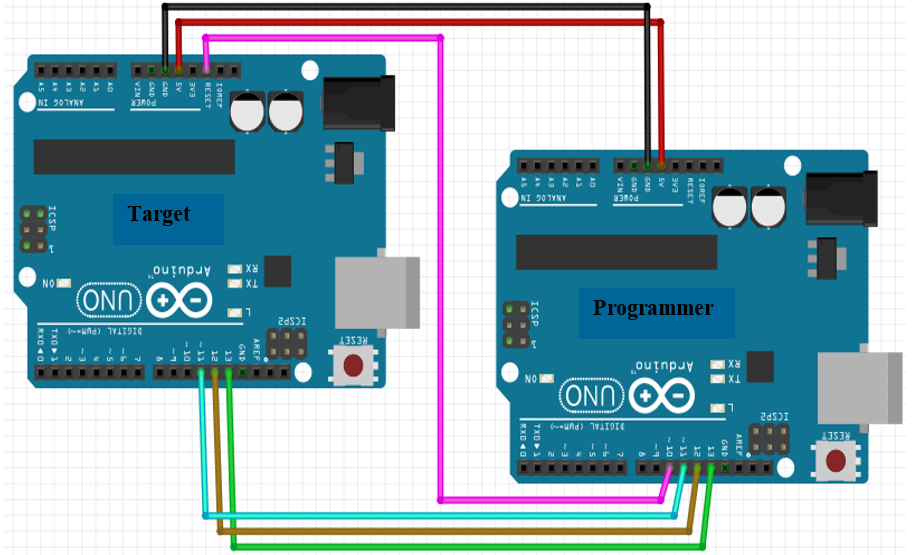
\includegraphics[scale=0.7]{EXP_14_Images/fig1.png}
\end{center}

\begin{center} {Figure 1. Arduino as an AVR-ISP Programmer}\end{center}



\item Now connect the Programmer to the PC.
\item Select the right port from the 'Tools' menu.
\item  Go to the Programmer in the 'Tools' and select 'Arduino as ISP'.
\item  Write any program, says, 'LED blinking connected at pin 7 of Target'.
\item Now go the 'Sketch' and choose 'Upload using programmer'.
\item Remove the communication and reset cables.
\item  Connect the LED to pin7 via a resister. See the result.  
\end{itemize}

\noindent Note: Programming via this method deletes the bootloader in the Target board and it cannot be programmed through USB directly. To program the target again via USB, connect as above again and go to the 'Tools' 'Burn the Bootloader'. Once the bootloader is burned in the target board it can be again programmed via USB.
\end{justify}

\vspace{40mm}
\textbf{\large REFERENCES:}
\vspace{-6mm}
\begin{enumerate}
\setlength\itemsep{-0.3em}
\item  \href {https://docs.arduino.cc/built-in-examples/arduino-isp/ArduinoISP}{ArduinoISP }

\end{enumerate}

\textbf{\large Concept Drills on Bare Metal Programming :}

\vspace{-6mm}
\begin{justify}
\begin{enumerate}
 \setlength\itemsep{-0.3em}
\item Three LEDs are connected to port C from PC2 to PC4. Write a program such that all LEDs remain ‘ON’ except the LED connected to PC3, which keeps blinking with a delay of 300ms.
\item Write a code using the XOR concept so that LED blink with a 1second delay normally but upon pushing the switch it starts blinking with a delay of 200 ms.
\item Using Timer 1 with a Prescaler value of 256, blink an LED connected to the 7th pin of Port D. Show the relevant calculation.
\item Use Timer 1 with a Prescaler value of 256. Blink an LED connected to the 7th pin of Port D by making a user-defined delay function using the timer flag concept. Show the relevant calculation.
\end{enumerate}
\end{justify}

\end{document}